%! suppress = FileNotFound
\documentclass[a4paper,12pt]{report}
\usepackage{graphicx}
\usepackage{hyperref}
\usepackage{float}
\usepackage{makecell}
\usepackage[nottoc]{tocbibind}

\pagestyle{headings}
\graphicspath{{./Images/}}
\hypersetup{
	colorlinks=true,
	linkcolor=blue,
	filecolor=magenta,
	urlcolor=cyan,
}


\begin{document}


\begin{titlepage}
	\begin{center}
		\vspace*{1cm}

		\Huge
		\textbf{Design Document - DD}

		\vspace{0.5cm}
		\large
		January 2021

		\vspace{1.5cm}


		\vfill

		
\includegraphics[scale=0.7]{PolimiLogo}

		\vfill


		\normalsize
		\textbf{KONG XIANGYI} \\
		\textbf{\&} \\
		\textbf{ZHANG YUEDONG}

	\end{center}
\end{titlepage}

\tableofcontents


\chapter{INTRODUCTION}\label{ch:introduction}


\section{Purpose}


\section{Scope}


\section{Definitions, Acronyms, Abbreviations}
\subsection{Definitions} \label{subsec:definitions}
\begin{itemize}
	\item Click Customer : The customer has the required technology to access the store.
							I.e a smartphone.
							They can use the customer terminal software.
	\item Brick Customer : The customer doesn't have the required technology to access the store, they have to hand out "tickets" on the spot.
	\item Store Manager : They have to manage the Store System, include the software and hardware.
	\item Ticket: The ticket is a document which contains three key information: QR Code, the estimated departure time, the queue number, and the Store Planned Roadmap.
					To the click customer, it's \textbf{E-ticket} but to the brick customer,it's \textbf{Paper Ticket},and doesn't contain the estimated departure time, and just a General Store Map without the Planned Road.
	\item QR Code : When customer booked a visit, they will received a QR Code.
	\item QR Code Scanned Machine : A hardware, the Click Customer can use this machine scan their QR code.
	\item Tickets Hand-Out Machine : A hardware, the Brick Customer can use it retrieve their Ticket.
	\item Store Planned Roadmap: A store map that includes a finer way which is recommended form Store System.
	\item Digital Counterpart : A hardware, it with show the queue number.
	\item Store Back-End System : A software, as the back-end manages all stuffs.
	\item On-Time Store Data : A dataset that includes the store's on-time date.
	\begin{itemize}
		\item The current queue
		\item The customers in the store
		\item The maximum number of people in the store.
	\end{itemize}
	\item Long-Term Customers: The Click Customer who visited the store more than one time by the CLup mobile application.
\end{itemize}


\subsection{Acronyms}
\begin{itemize}
	\item RASD - Requirement Analysis and Specification Document
	\item DD - Design Document
	\item CLup - Customers Line-up
	\item UI - User Interface
	\item IOS - iPhone OS
	\item PC - Personal Computer
	\item IaaS - Infrastructure as a Service %TODO delete IaaS
	\item CRM - Customer Relationship Management
	\item LAN - Local Area Network
\end{itemize}


\subsection{Abbreviations}
\begin{itemize}
	\item %TODO
\end{itemize}


\section{Revision history}


\section{Document Structure}


\chapter{ARCHITECTURAL DESIGN}\label{ch:architectural-design}

In this chapter, we will describe the architectural design of our system.

We will use the Top-down design approach, design the very high-level structure first,
and then gradually work down to detailed decisions about low-level constructs.
Finally, arrive at detailed decisions.\cite{Slides}
Let us start with the High-level components and their interaction.


\section{Overview: High-level components and their interaction}\label{sec:ArchitectureOverview}

We chose \textbf{3-Tiered architecture} with the \textbf{Thin Client} strategy for our system.
As shown in Fig.\ref{fig:ThreeTieredArchitecture}.\cite{SistemiInformativi}

\textbf{Tier-1} is the presentation layer.
This layer will deploy the Click Client's mobile application,
Store Manager's Management Web Page, and even Digital Counterpart and Ticket Hand-Out Machine's presentation.

\textbf{Tier-2} is the logic application layer.
This layer will deploy our Back-End System component.

\textbf{Tier-3} is the data access layer.
This layer includes our DBMS and the Data Base.

We have a web page as the Management page for the Store Manager but considered this page a static page, and the traffic will be minimal,
so we did not use the 5-Tiered Architecture with the Web Server and the Script Engine Server to general the Dynamic Page.

Finally, our high-level architecture is shown in Fig.\ref{fig:HighLevelArchitecture}.
The Store Manager's PC and other hardware will connect with an Ethernet cable.
The Click Customer's Mobile App communicates with our Back-End System with the Internet.

More detailed components will be introduced in the next section.


\begin{figure}
	\centering
	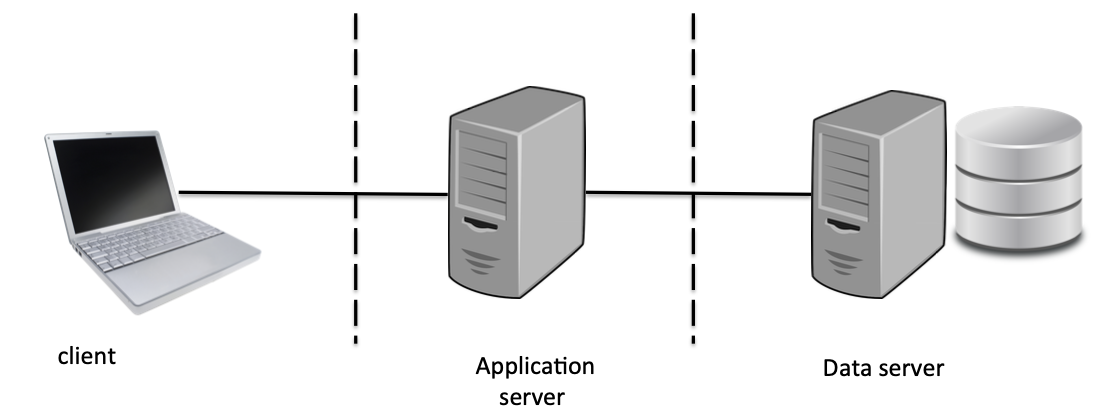
\includegraphics[scale=0.7]{ThreeTiered}
	\caption{3-Tiered architecture}
	\centering
	\label{fig:ThreeTieredArchitecture}
\end{figure}

\begin{figure}
	\centering
	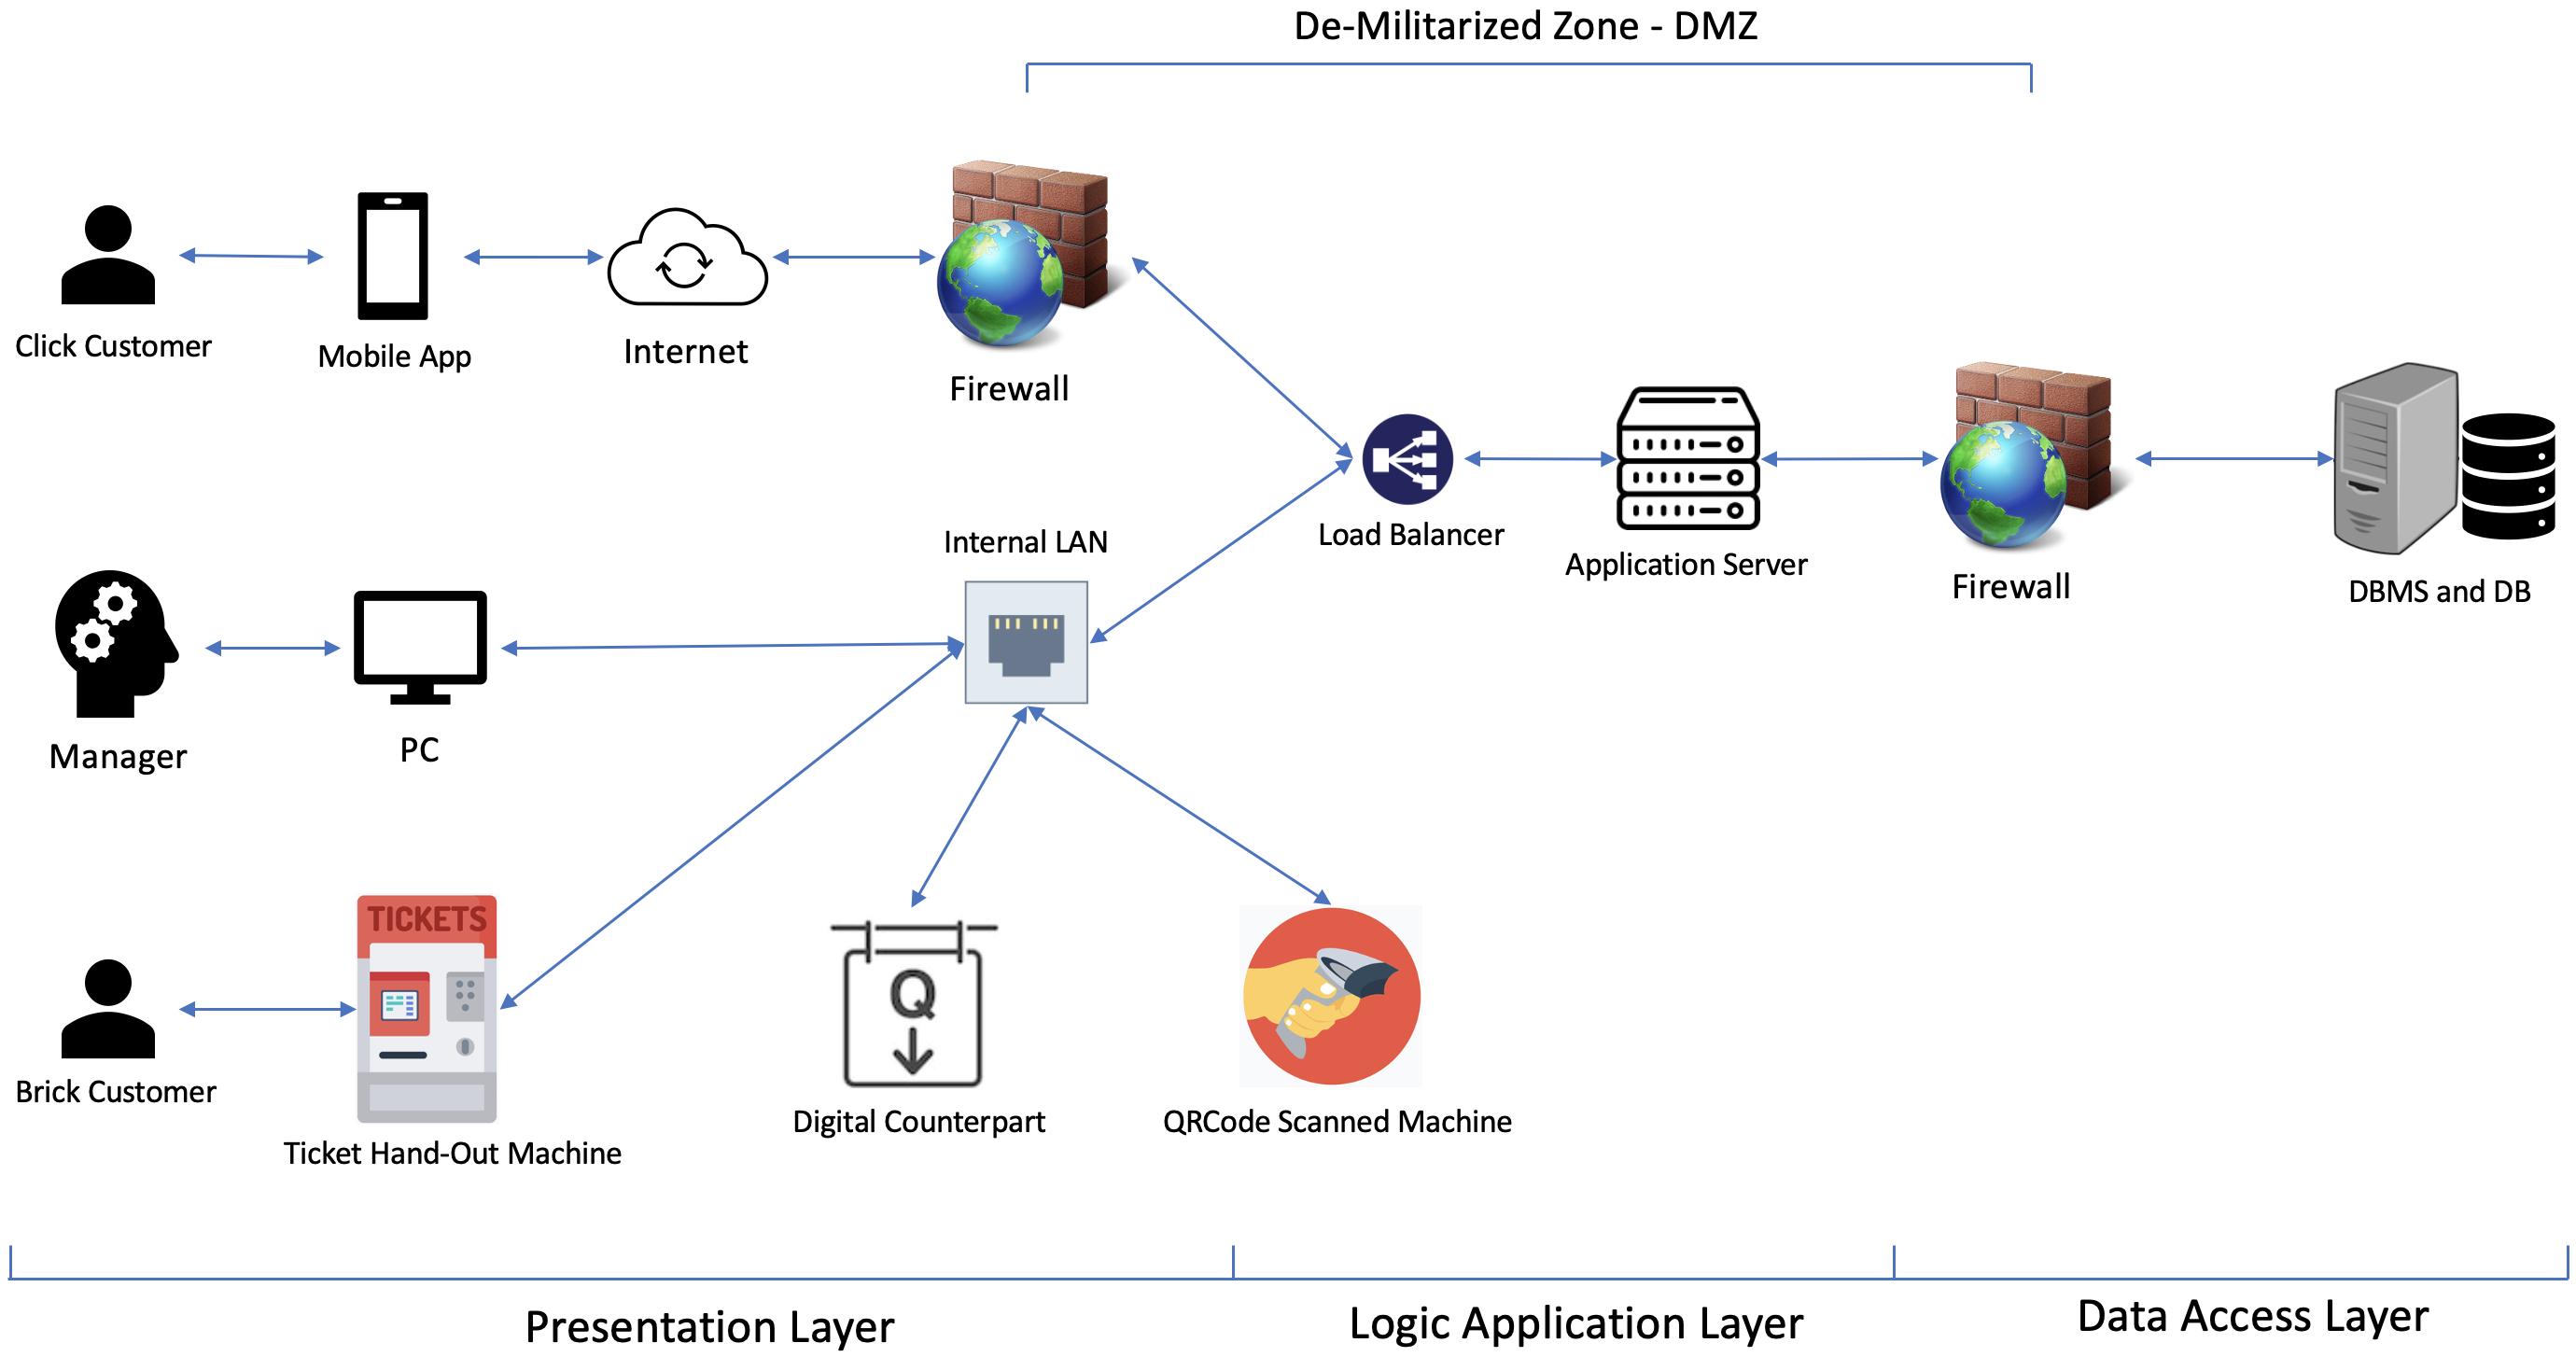
\includegraphics[scale=0.37]{HighLevelArchitecture}
	\caption{High level architecture}
	\centering
	\label{fig:HighLevelArchitecture}
\end{figure}

\section{Component View} \label{sec:ComponentView}
The following diagram Fig.\ref{fig:ComponentDiagram} is the \textbf{Component Diagram}, and it contains all components in our system.
This diagram shows the 3-Tiered Architecture of our system.
The Yellow components are in Presentation Layer.
The blue components are in the Logic Application Layer, and the Green components DBMSServer is in the Data Access Layer.
We will separately introduce all these components in this section and introduce all interfaces at Sec.\ref{sec:component-interfaces}.

The \textbf{Redirector} component is a bridge for communicating the Presentation Layer and the Logic Application Layer.
It is transparent to User and back-end systems, plays the role of forwarding information on both sides, and connect interfaces.
It has four subsystems, respectively, responsible for communicating with four types of devices, as shown in Fig.\ref{fig:component_diagram_redirector}.

The \textbf{ClickCustomerRedirector} will transfer the message between Mobile Application and the Application Server.
The Register message will pass by the RegisterNewClickCustomer, and look out the Valid/History Booking will use the GetClickCustomerData Interface,
this Interface will return all information of this Customer.
For the most important operation - Booking a visit, use GetBookingSchedule to get the available Time/Date.
Then, through the ModifyClickCustomerData Interface to submit the Booking,
by the way, it also can modify other available data of this Customer.
Moreover, the SendNotifyToClickCustomer Interface will handle Notify message.
The Mobile Application can actively "pull" Notify message through this Interface from the Back-End System.
To "push" Notify information, we will use the Observer Pattern.
It will introduce in Sec.\ref{sec:SelectedArchitecturalStylesAndPatterns}

The \textbf{TicketMachineRedirector} will transfer the Ticket Hand-Out Machine's message.
It needs two pieces of information, the allowed \hyperref[subsec:definitions]{maximum number of people in the store} and how many Customers in the Queue in time.
So The GetQueueSchedule and GetMaxNumberInStore Interface can do these operations, and these two fields will show on the Ticket Machine's screen.
Finally, the retrieve ticket operation will handle by the ModifyQueueSchedule Interface.
It will put a BrickCustomer into the Queue.

The \textbf{DigitalCounterpartRedirector} will help the \hyperref[subsec:definitions]{Digital Counterpart} display the next queue number.
The Customer can enter the store after found his number on the Digital Counterpart.

The \textbf{ManagementSystemRedirector} will function for the Management System of our Store Manager.
This redirector will transmit the message between the Presentation layer's web page and the Back-End System.
Through the Interface shown in Fig.\ref{fig:component_diagram_RedirectoSubsystem}, the Manager can realize his operation like reschedule someone's Booking, adjust the Queue order, or lower the maximum number.

The next three subsystems are the core subsystems in our application layer.


\begin{figure}
	\centering
	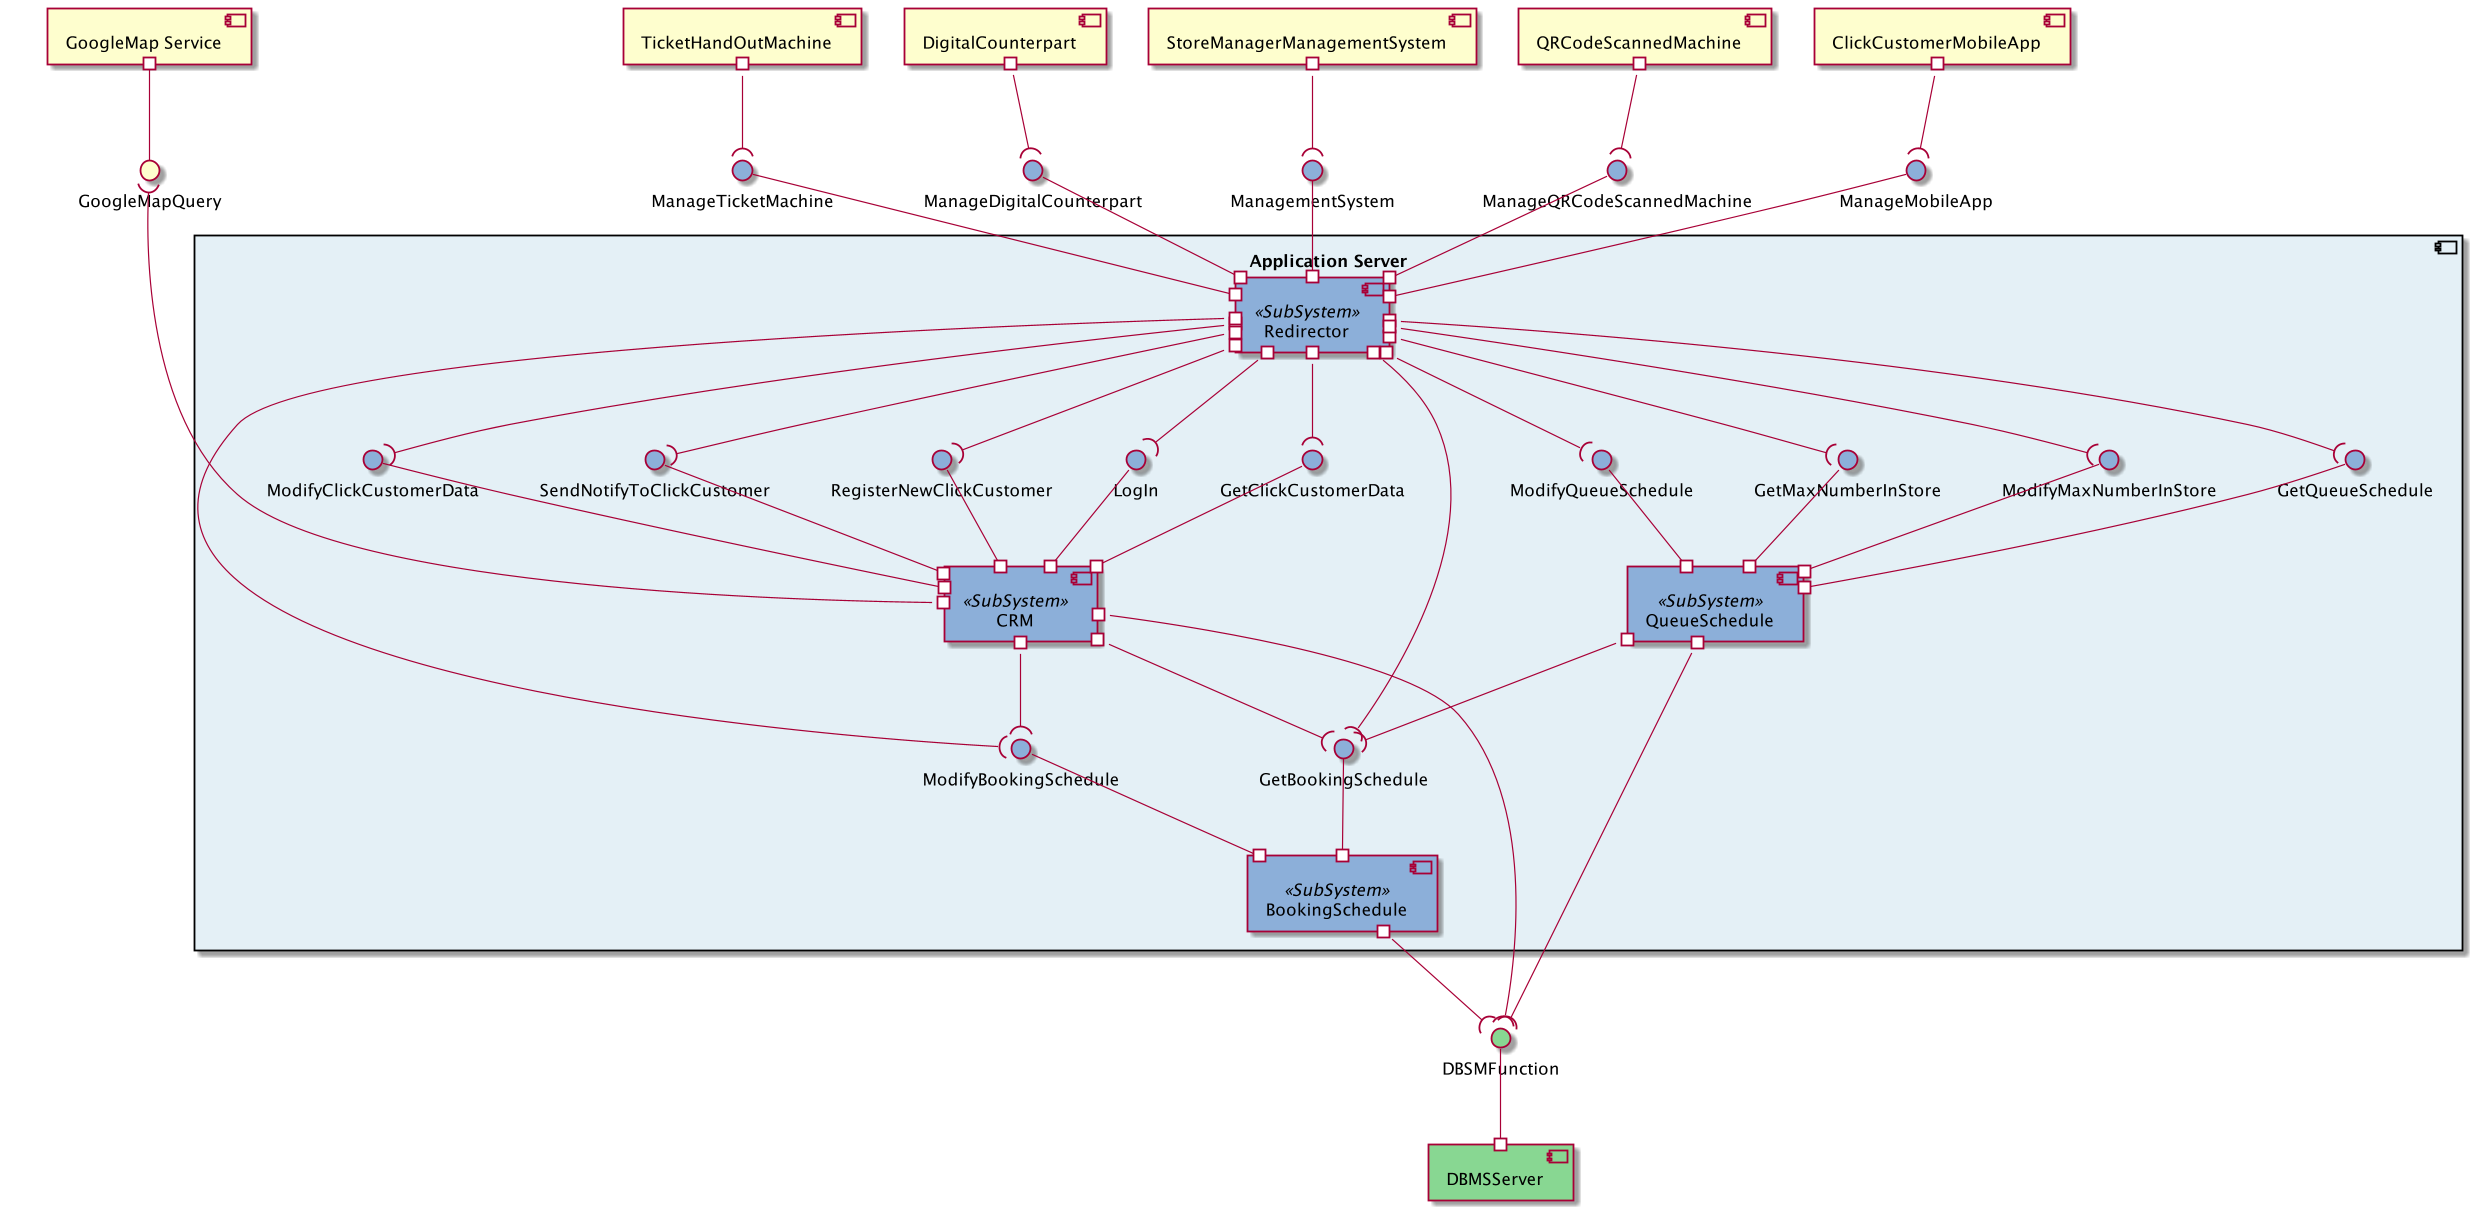
\includegraphics[scale=0.16, angle=270]{component_diagram}
	\caption{Component Diagram}
	\centering
	\label{fig:ComponentDiagram}
\end{figure}

\begin{figure}
	\centering
	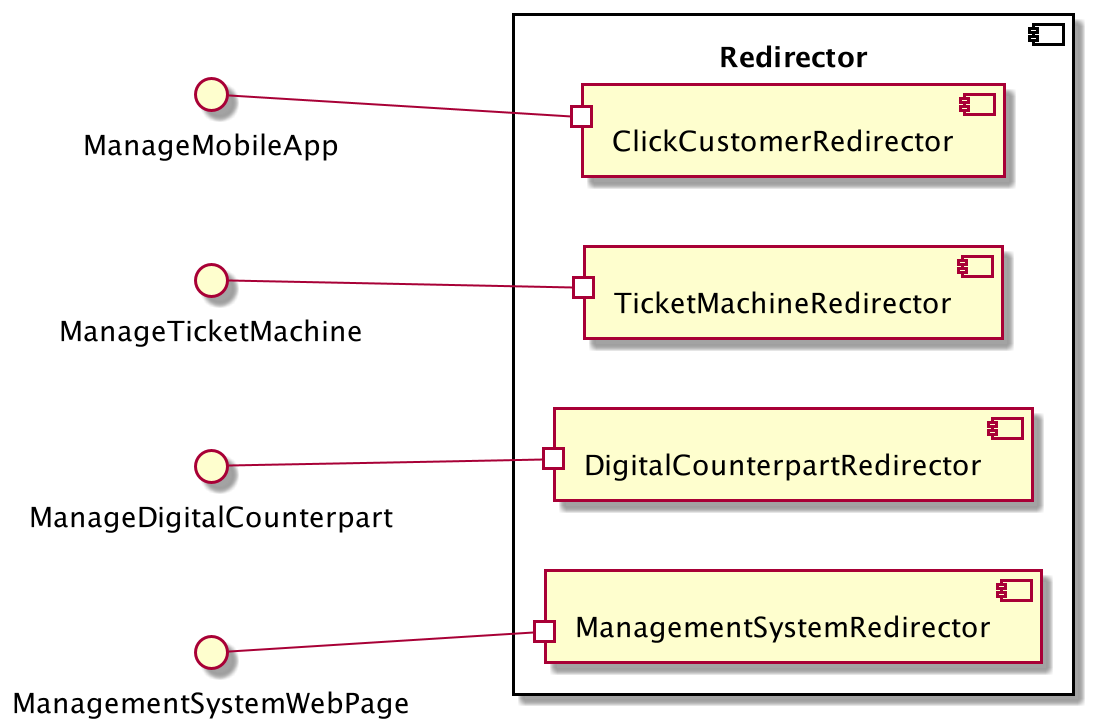
\includegraphics[scale=0.3]{component_diagram_redirector}
	\caption{Redirector Component Diagram}
	\centering
	\label{fig:component_diagram_redirector}
\end{figure}

\begin{figure}
	\centering
	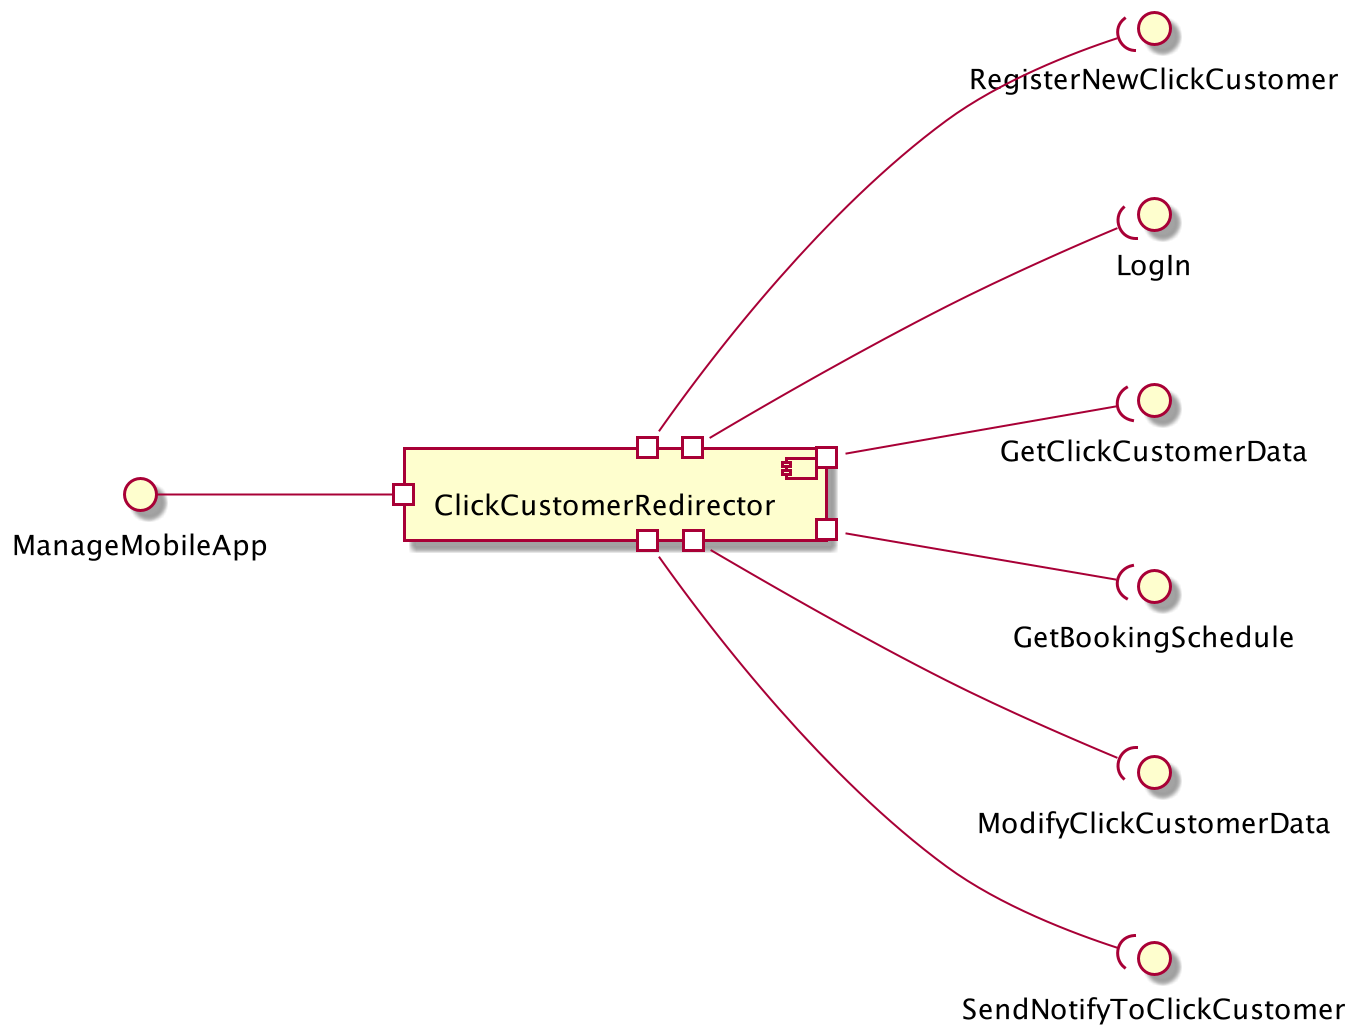
\includegraphics[scale=0.2]{component_diagram_ClickCustomerRedirector}
	\vspace{10mm}
	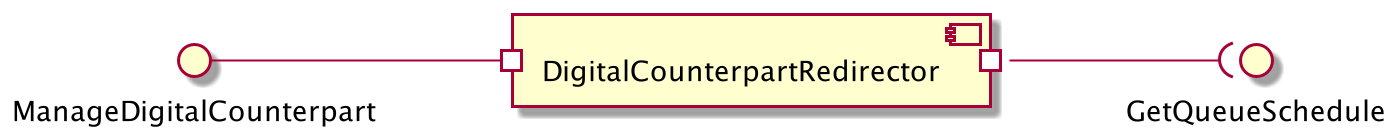
\includegraphics[scale=0.2]{component_diagram_DigitalCounterpartRedirector}
	\vspace{10mm}
	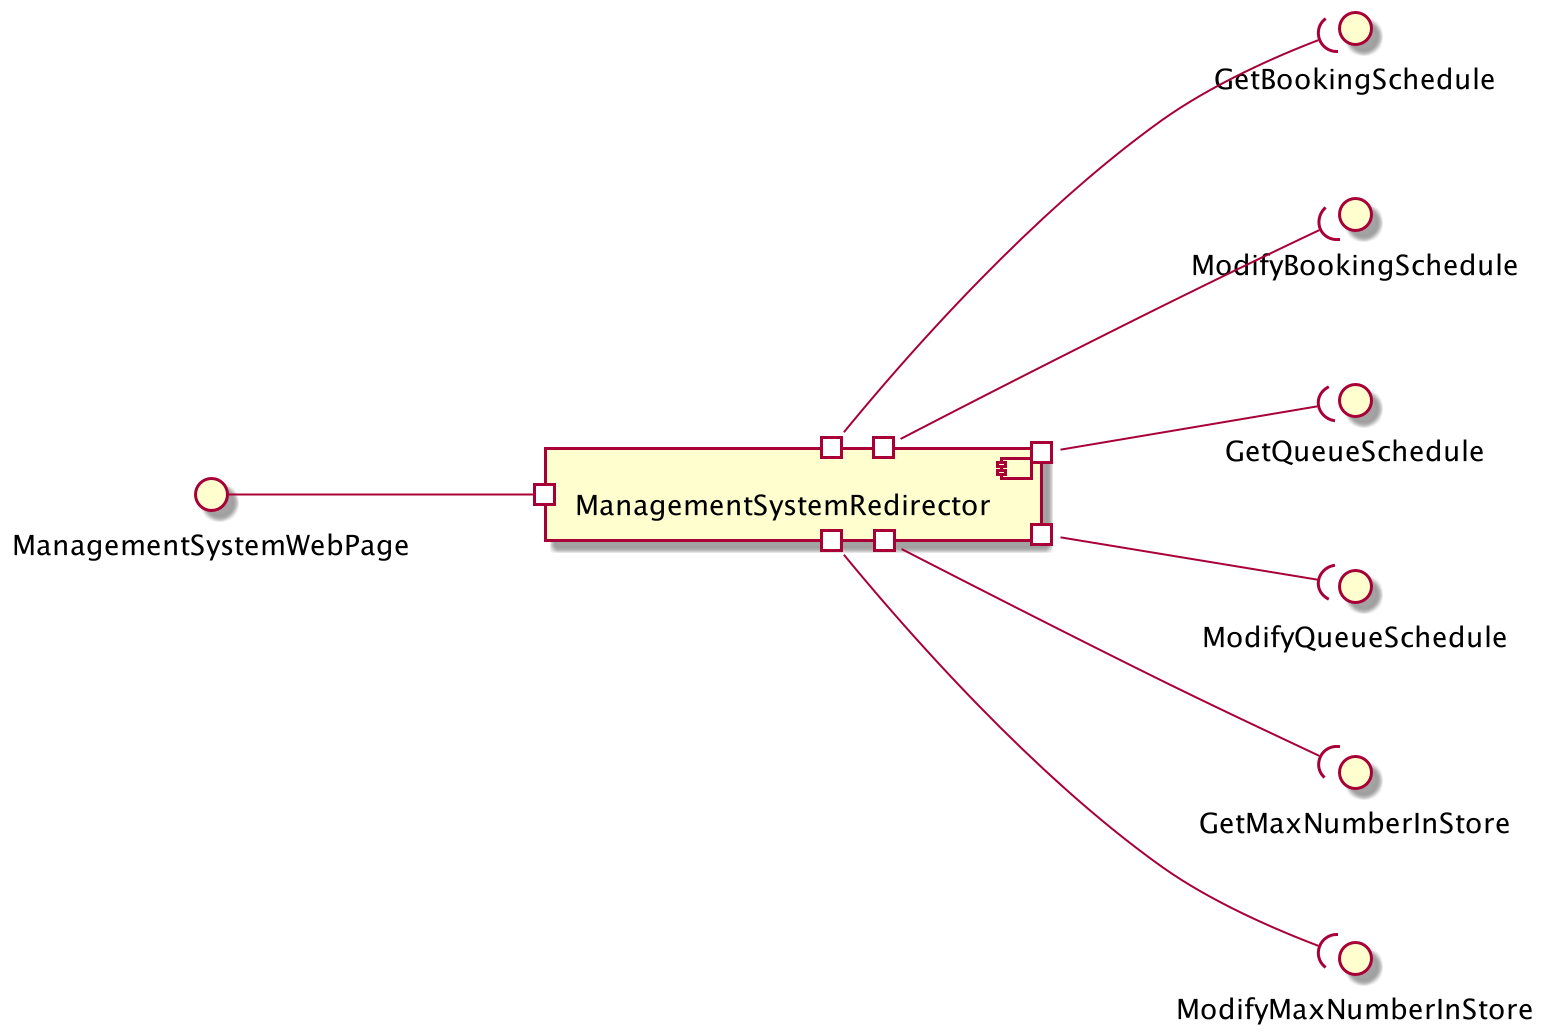
\includegraphics[scale=0.2]{component_diagram_ManagementSystemRedirector}
	\vspace{10mm}
	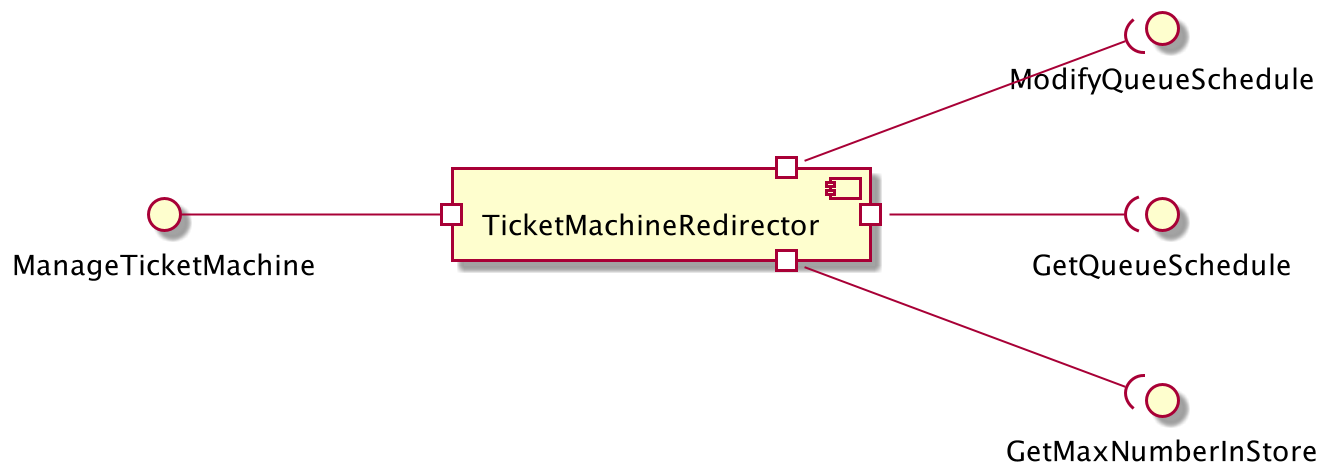
\includegraphics[scale=0.2]{component_diagram_TicketMachineRedirector}
	\vspace{10mm}
	\caption{Redirector's Subsystem Component Diagram}
	\centering
	\label{fig:component_diagram_RedirectoSubsystem}
\end{figure}

\section{Deployment View}




\section{Runtime View}



\section{Component Interfaces}\label{sec:component-interfaces}


\section{Selected Architectural Styles and Patterns}\label{sec:SelectedArchitecturalStylesAndPatterns}

%MVC
%Observer Pattern

\section{Other Design Decisions}

\chapter{USER INTERFACE DESIGN}\label{ch:user-interface-design}


\chapter{REQUIREMENTS TRACEABILITY}\label{ch:requirements-traceability}


\chapter{IMPLEMENTATION, INTEGRATION AND TEST PLAN}\label{ch:implementation-integration-and-test-plan}


\chapter{Effort Spent}

\begin{itemize}
	\item \textbf{Kong XiangYi}
	\begin{center}
		\scalebox{0.8}{
			\begin{tabular}{ |c|c|c| }
				\hline
				Date & Task & Hours \\
				\hline
				\hline
				2021/01/02 & Group discussion and task assignment & 2h \\
				\hline

		\end{tabular}}
	\end{center}


	\item \textbf{Zhang YueDong}
	\begin{center}
		\scalebox{0.8}{
			\begin{tabular}{ |c|c|c| }
				\hline
				Date & Task & Hours \\
				\hline
				\hline
				2021/01/01 &  Launch DD  & 2h \\
				\hline
				2021/01/02 & Group discussion and task assignment & 2h \\
				\hline
				2021/01/03 & Did S.\ref{ch:architectural-design}.\ref{sec:ArchitectureOverview}
				and S.\ref{ch:architectural-design}.\ref{sec:ComponentView}
				Component Diagram & 3h \\
				\hline
				2021/01/04 & Did S.\ref{sec:ComponentView}.
				Component Diagram describe. & 2h \\
				\hline
			\end{tabular}}
	\end{center}
\end{itemize}




%Bibliographic references
\begin{thebibliography}{9}

\bibitem{SistemiInformativi}
Cinzia Cappiello, Mariagrazia Fugini, Paul Grefen, Barbara Pernici, Pierluigi Plebani, Monica Vitali. (7 settembre 2018)  Fondamenti di Sistemi informativi: per il Settore dell'Informazione.

\bibitem{IEEESDD}
"IEEE Standard for Information Technology--Systems Design--Software Design Descriptions," in IEEE STD 1016-2009 , vol., no., pp.1-35, 20 July 2009, doi: 10.1109/IEEESTD.2009.5167255.

\bibitem{IEEEAD}
"ISO/IEC/IEEE Systems and software engineering -- Architecture description," in ISO/IEC/IEEE 42010:2011(E) (Revision of ISO/IEC 42010:2007 and IEEE Std 1471-2000) , vol., no., pp.1-46, 1 Dec.
2011, doi: 10.1109/IEEESTD.2011.6129467.

\bibitem{Slides}
Elisabetta Di Nitto, Matteo Rossi. (A.Y.2020/2021) The slides of the Software Engineering 2 course.

\end{thebibliography}


\end{document}

